\chapter{Ontologies} \label{ch:ontologies}

\todo{This is an easy story to tell if you walk through the
slides from your last committee meeting, and then answer any remaining
questions below.}

A formal system for describing scientific workflows would be valuable for a
variety of reasons. Perhaps most importantly, this includes being able to
determine what types of systems need to be implemented to successfully execute
the workflow. This is fundamentally a question about our ability to model our
workflows thoroughly without building out a fully functional system, which is
common at present. It is not clear that this model will continue to scale up
efficiently as workflows become more distributed, hierarchical, and mixed
because of the associated increase in complexity. 

One important tool in understanding complex computing systems is an ontology.
An ontology captures knowledge about a system in a formal way. This includes
capturing details about entities, classes of entities, entity properties, and
the relationships between these things. Ontologies are usually recorded in a
graph data structure. The graph can be modified, linked, or merged with other
ontology graphs to create an even greater understanding of a topic.

This chapter introduces ontologies with a focus on how they can be used to
better understand different types of workflows, workflow management systems,
and workflow data models. First, common properties of ontologies are reviewed to
provide a basic understanding of their use. Second, a short example is provided
to illustrate their use in encoding real-world data. This includes an
illustration of why ontologies are sometimes favored over taxonomies. Finally, a
common set of tools for working with ontologies is presented to illustrate how
ontologies are created in formal ways that are machine-readable, ready for
distribution, and use in larger applications.

*Why do ontologies matter here?

*Ontology versus taxonomy

*How can this be written in plain text, without invoking RDF?

*What does this look like in RDF?

*What is RDF?

*What is the semantic web?

*How does this jive with scientific workflows?

\section{Features of Ontologies}

Ontologies are commonly described using special ontology languages, such as the
Web Ontology Language (OWL), or modeling languages like the Unified Modeling
Language (UML). There are a number of common features found across these
languages, some of which are useful for the following discussions. 

\subsection{Properties}

Entities in an ontology can have properties that describe their makeup. Some
entities, such as primitive double precision floating point numbers have their
value as their only property. However other entities, such as a computer, may
have many properties including hardware peripherals and non-physical properties
including cost. Entities are connected to properties through relationships.

\subsection{Objects and Classes}

An object is a specific entity that has been initialized with some default.
A simple equation $x = 5$ could be used to denote that the object $x$ has the
value five. A set of objects is defined by a class. Objects may sometimes be
called instances or individuals, and all three terms are used interchangeably
herein.

Classes define the properties (or in some definitions links to properties) and
required relationships for objects. One special relationship is the
\textit{Inheritance} relationship. This relationship indicates that one class
must have - inherit - the properties and relationships of another class, called
its ``parent.'' Classes that inherit from other classes are said to be
subclasses of their parent ``base'' class.

A trivial example would be a class Money with subclasses Coin and Bill. In
United States Currency, Coin would have subclasses Nickel and Penny. A roll of
pennies from a bank would contain fifty pennies, all of which would be objects
or insances of the Penny base class.

\subsection{Ontological Openess}
\label{ont-openess}

Ontological openess is the quality of a graph to be left open to modification.
Open ontologies are capable of describing knowledge from multiple perspectives
that more accurately describe the nature of the object. It is possible for
individual entities within the ontology to be modified, or for new graphs to be
linked to the existing graph to provide these different perspectives.

Consider, for example, a tea cup. What is it? Is it a vessel for holding tea or
is it clay? Is it plastic? Is it red, blue, or covered with a picture of
Captain Picard? Was it a gift? Is it warm to the touch? Is it also possible to
hold other liquids? By leaving an ontology that only describes what the tea cup
can hold open to extension, all of these properties can be linked to describe a
clay tea cup that can also hold coffee, that has a picture of Captain Picard on
it, that was a gift, and which was warm when the author started writing this
page.

\section{Case Study: A professor, a businessman, and a pilot}
\label{case-study}

It is straightforward to create an educational example of an ontology that is
also simple enough to be easily understood. The example below considers the
members of a thesis committee for which all six of the following statements are
true:

\begin{enumerate}
\item Mike, Mike Jr., and Jack are full professors. %1
\item John T. and Arjun are adjunct professors.     %2
\item John D. is a research professor.              %3
\item Mike is also a businessman and a pilot.       %4
\item Mike Jr. is Mike's son.                       %5
\item Mike and John both play guitar.               %6
\end{enumerate}

The goal of the exercise is to encode all six of these statements into a single,
formal ontology that is easily understood by the reader.

For pedagogical reasons that will become evident throughout the discussion, it
is first useful to attempt to organize this information as a simple taxonomy, a
tree structure with one simple ``is'' relationship. In fact, this is a natural
and obvious choice because most of the statements indicate that the members of
the committee ``are'' professors, etc. Taxonomies are commonly understood as
tools used to organize families, including family trees in genealogy.

Statements 1-3 in the list describe six indivuals who are all professors.
However, three distinct types of professors are listed. Since there is no
statement saying otherwise, it is reasonable to assume (and in fact correct),
that the terms full, adjunct, and research professor all describe separate types
of professors. That is, full, adjunct, and research professors are professors
(inheritance), and an individual may only be either a full, adjunct, or research
professor. The latter statement means that full, adjunct, and research
professors are \textit{disjoint}. 

Figure \ref{tax-1} shows a depiction of a simple taxonomy that clearly
illustrates the type of professor for most of the individuals. This taxonomy
shows a family of professors and is two levels deep. However, this figure only
encodes a few of the facts described above. One professor, Mike Jr., is missing,
and statements 4-6 are not considered.

\begin{figure}[htbp]
\centering
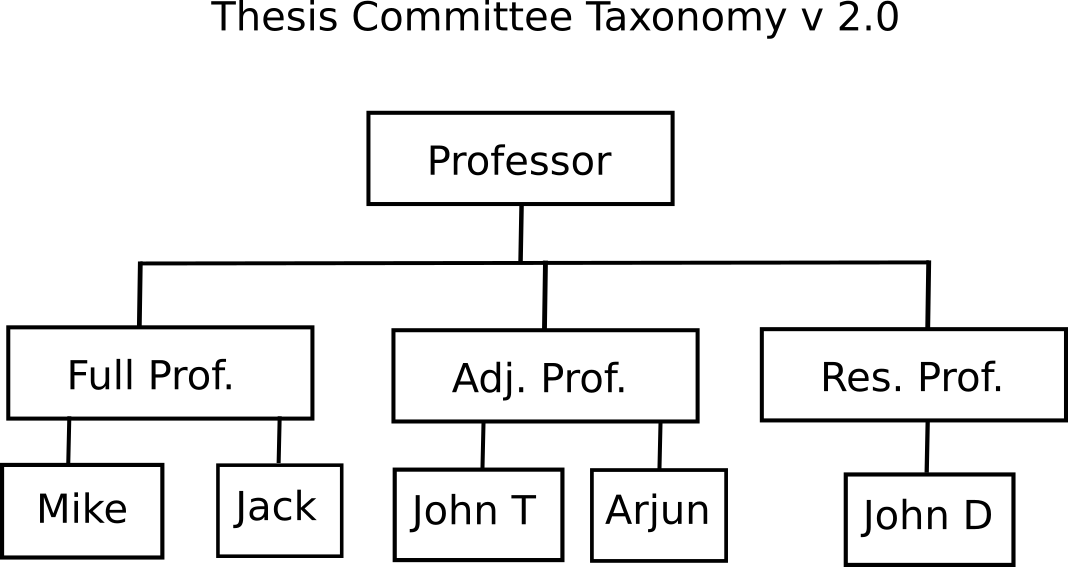
\includegraphics[width=\textwidth]{figures/tc-tax-v2.png}
\caption{A simple taxonomy of the the professors and their ranks as described
in \S \ref{case-study}.}
\label{tax-1}
\end{figure}

Figure \ref{tax-2} includes the facts from all six statements. The red ``X''
marks in this figure indicate where the single relationship rule of a taxonomy
has been broken. First, in a taxonomy all guitarists would inherit from the same
parent, or from multiple guitar-playing parents who inherit from another
guitar-playing grandparent. Second, although Mike Jr. is Mike's son, Mike Jr.
and a full professor, Mike Jr. is not a businessman and a pilot. Finally, the
relationship types between the professors, their bases classes, and the
additional occupational and familial classifications change throughout the
taxonomy in an unclear way.

\begin{figure}[htbp]
\centering
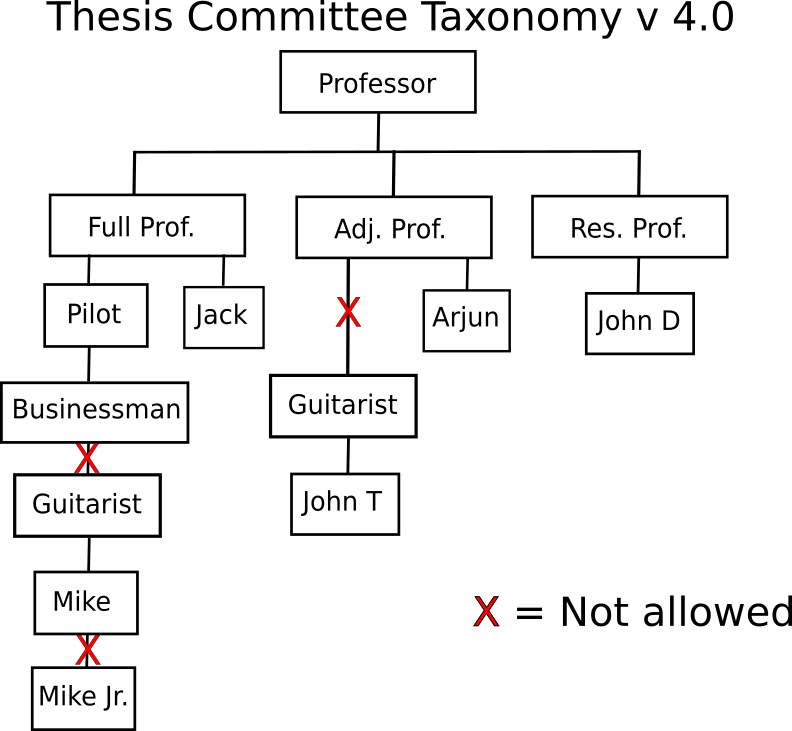
\includegraphics[width=\textwidth]{figures/tc-tax-v4-wErrors.png}
\caption{A ``complete'' attempt at encoding the facts in \S \ref{case-study}.
The red ``X'' marks indicate the types of relationships that are not allowed
under the rules of a taxonomy.} 
\label{tax-2}
\end{figure}

These issues illustrate the fundamental problem with a taxonomy for
heterogeneous knowledge capture: ``Basic'' taxonomies only allow single direct
inheritance relationships to be expressed. This can be partially fixed by
allowing the relationship type to be changed based on an in-line annotation, but
what about properties such as ``can play guitar?'' Conceptually ``can play
guitar'' is not the same type of relationship as an ``is-a'' relationship. Is
a special annotation or graphic required for each new property type?
Furthermore, how does one rectify the fact that not all full professors are in
business, fly planes, or play guitar? What if a research professor did those
things as well? The complexity of the required modified taxonomy creates such a
complex diagram that one might as well simply leave the statements written
instead of encoded!

As more changes to the fundamental taxonomic data structure are required, the
required formality and bookkeeping also increase. It quickly becomes necessary
to create a separate structure simply for the purposes of managing all the
bookkeeping. Then, the data structure that uses the bookkeeping data structure
becomes something that uses the bookkeeping relationships to encode the facts.
A complex bookkeeping structure of this type that can encode classes,
relationships, and properties is an ontology, and the accompanying structure,
the graph of individuals, is known commonly as an \textit{instance graph},
\textit{knowledge graph}, or just graph of members or instances of the
ontology.

A simple ontology that describes the types of relationships, properties, and
classes for the six statements above is shown in figure \ref{ont-classes}.
Notice that this ontology contains a simple taxonomy of classes who are
Persons. Unlike the original taxonomy, Businessman, Guitarist, Pilot,
and Professor are all peers. The ontology has the following properties:
\begin{itemize}
  \item isFullProf - individuals with this property are Full Professors
  \item isAdjProf - individuals with this property are Adjunct Professors
  \item isResProf - individuals with this property are Research Professors
  \item hasSon - individuals with this property have a son whose identity is the
  object of the property
\end{itemize} 
The isFullProf, isAdjProf, and isResProf properties are all boolean properties
that are either true or false. The \textit{hasSon} property is somewhat special
compared to the others because it encodes a relationship as a property. These
types of properties need to indicate clearly where they originate in the graph
and where they end. For statement 5 this could be indicated on the instance
graph by a property with a value of ``Mike Jr.'' or a graphic indication linking
Mike and Mike Jr.

The ontology also has the following \textit{disjoint} properties:
\begin{itemize}
  \item isFullProf != isAdjProf
  \item isFullProf != isResProf
  \item isAdjProf != isResProf
\end{itemize}
where the ``!='' indicates a negation relationship meaning ``is not.'' The
disjoint properties constrain the relationships between the normal properties
for semantic purposes. Subclasses are usually disjoint.

\begin{figure}[htbp]
\centering
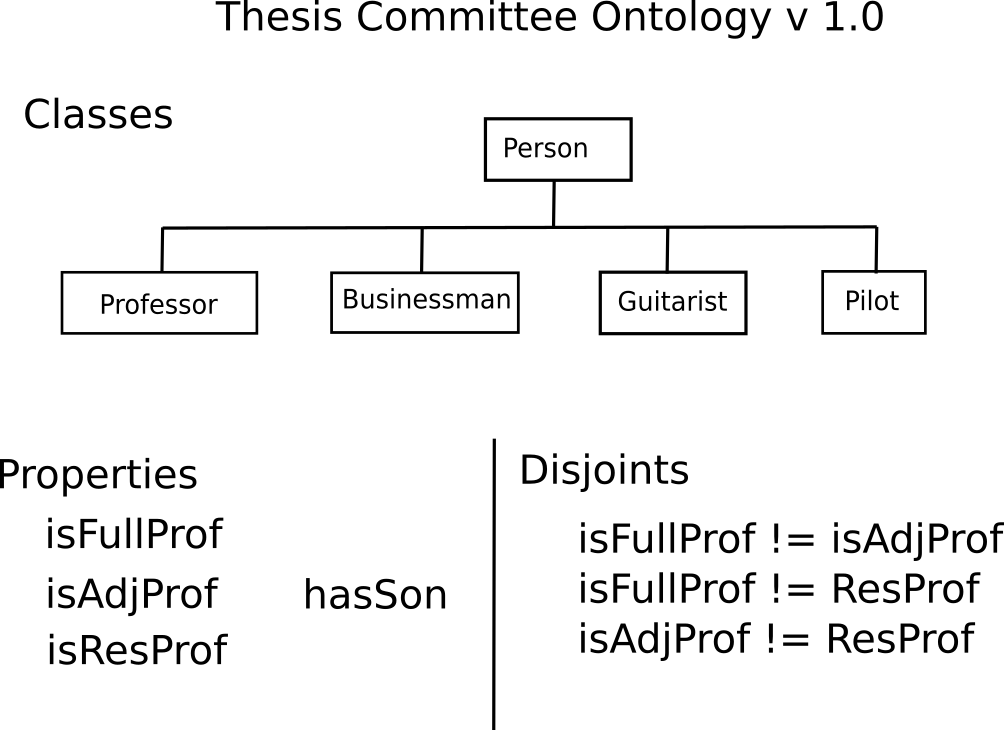
\includegraphics[width=\textwidth]{figures/tc-ont-classes.png}
\caption{The relationships, properties, and classes for the example of \S
\ref{case-study}.}
\label{ont-classes}
\end{figure}

The instance graph that uses the ontology to encode all six statements is shown
in figure \ref{ont-instances}. This graph combines taxonomic ``is-a''
relationships and the ontological properties to fully represent the facts,
and removes the representational problems found in figure \ref{tax-2}. This
includes Mike's multiple roles and parental status. Professorial rank is
captured with properties instead through direct inheritance. Note that the
green line in this figure has no special significance, but it's color is useful
to show its path next to the black lines.

\begin{figure}[htbp]
\centering
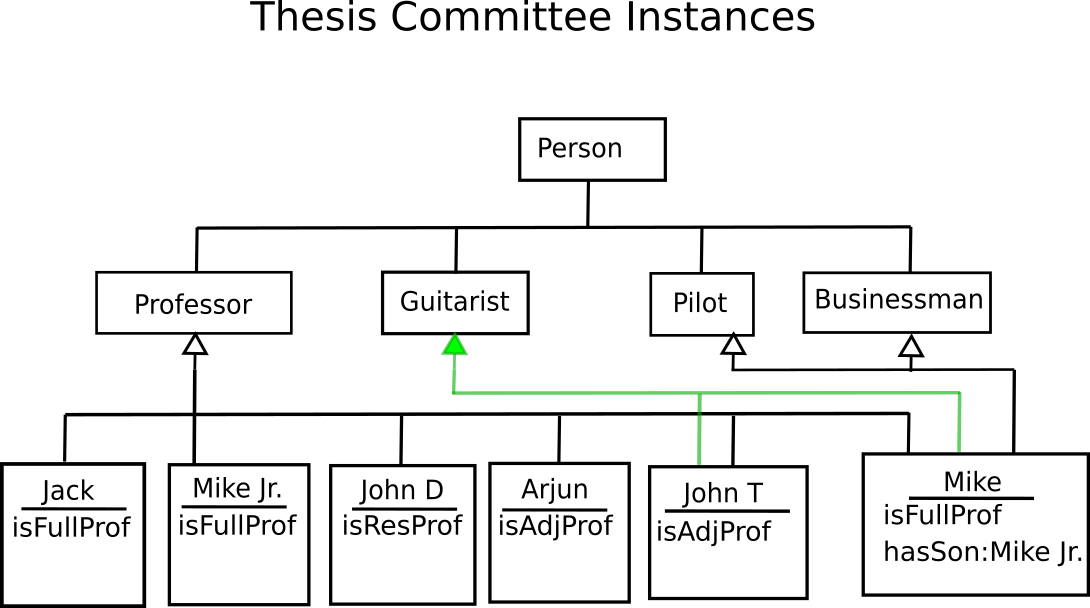
\includegraphics[width=\textwidth]{figures/tc-ont-instances.png}
\caption{The instance graph that uses the ontology in figure \ref{ont-classes}
to encode the example of \S \ref{case-study}. The green line is not of
ontological signficnance, but colored separately to show the full connection.}
\label{ont-instances}
\end{figure}

An important aspect of ontologies, including this example, is new facts that
are not present in the instance graph can often be inferred from the facts that
are present. Alternatively, because the graphs are open, merging graphs can
reveal new facts when inference rules are applied. Two facts than can be
inferred from the present set of facts is that an inverse relationship exists
for ``hasSon,'' which we might obviously call ``hasFather,'' and the identity of
Mike Jr.'s father is Mike. These facts are obvious to human readers, but that is
only because our experience fills in the ontological gaps. With respect to graph
mergers revealing new facts, suppose that someone merged a new ontology that
described Persons in great detail, and that one property it described is that
all sons are male. It would then be possible to immediately deduce that Mike Jr.
is male.

\section{Machine Readable Ontologies}

Real life ontologies are significantly more complex than the example in \S
\ref{case-study}. They are also used to capture and reason about large sets of
facts, which requires computational resources for processing. It is not feasible
to create any such ontology using the scheme in the example, and numerous
ontological standards have been developed. 

The Web Ontology Language (OWL) and related languages are used for this work to
capture ontological details in a machine readable way without sacrificing any
formality that is also useful to the human reader. OWL is based on the Resource
Description Framework Schema, which is in turn based on the Resource
Description Framework.

Summaries of these languages are provided below based on the most recent
langauge specifications and other sources, \cite{allemang_semantic_2008}. These
summaries also include practical findings from the author who as a user of these languages
discovered a number of pitfalls that are not commonly or widely discussed in the
extant literature.

\subsection{The Resource Description Framework}

The Resource Description Framework (RDF) is  W3C Standard for exchanging data
across the internet, \cite{rdf-w3c,rdf-concepts-syntax}. It forms the basis of a
so-called \textit{semantic web} where data resources are both linked and
self-describing, thus making large knowledge graphs that can be easily walked
to understand and find meaning in data.

The key concept in RDF is that statements can be made about uniquely
identifiable \textit{resources} in human and machine readable ways. Resources
are uniquely identified with Internationalized Resource Identifiers (IRI) that
extend the Universal Resource Identifier standard by adding support for
non-English characters and non-ASCII character sets. Resource names can be
anything from simple names that are locally unique to fully qualified globally
unique names.

Descriptions of resources are made with statements. Statements in RDF are
similar to sentences in the English language. Each statement contains a subject,
predicate, and object. The predicate describes the relationship of the subject
to the object in an RDF statement just as the predicate (verb) ``is`` links the
subject ``color'' (or ``ballColor'') to the object ``red'' in ``The color of
the ball is red.'' This type of statement is called a \textit{triple}.

RDF triples are represented as full graph data structures in memory, and
serialized to any one of a number of file formats, including an XML-based format
and several formats that are easier for humans to read, \cite{rdf-wikipedia}.
Most of the supported formats for RDF are standardized, although several formats
add support for additional features not found in the standard. This includes the
JSON Linked Data (JSON-LD) and Notation3 (Notation3) formats. Unless otherwise
specified, the remainder of this document will use a very readable and common
serialization called the Terse RDF Triple Language (TURTL), \cite{turtl}. This
format is signifcantly easier to understand than others for humans, and has the added
advantage of being succinct in written text. For example, the statement ``The
color of the ball is red'' would be rendered as a TURTLE triple with
\begin{lstlisting}
<#ball>
    hasColor <red>.
\end{lstlisting}
where as an RDF/XML triple it would be
\begin{lstlisting}[language=XML]
<?xml version="1.0"?>
<RDF>
  <Description about="ball">
    <hasColor>red</hasColor>
  </Description>
</RDF>
\end{lstlisting}

Statements about resources can be distributed, including outside of the
present graph. In the RDF literature, this is described by the
phrase ``Anyone can say anything about anything'' (AAA). This means that for any
given resource, any other resource can be included in triples. This is akin to
the ontological openess described in \S \ref{ont-openess}. This also means that
without human intervention it is very hard to establish the origin of data
for which there are numerous distributed triples, unless one of those
triples provides such a description. Within the current graph, resource
descriptions can be segmented for clarity. If a statement such as ``Jay Jay
Billings works at Oak Ridge National Laboratory, a DOE facility,'' is made,
instead of writing a single TURTL triple that captures all the facts, it
could be written as
\begin{lstlisting}
<#JayJayBillings>
    worksAt <#ORNL>.
<#ORNL>
    a <#NationalLaboratory>;
    hasName ``Oak Ridge National Laboratory''^^xsd:string.    
\end{lstlisting})
which uses references to other triples and links them into the original
triple about the author.

Notice the previous listing includes the term
\begin{lstlisting}
    hasName ``Oak Ridge National Laboratory''^^xsd:string.
\end{lstlisting}
This term assigns a \textit{literal} value of ``Oak Ridge National Laboratory''
to the subject of the triple. The additional characters at the end -
``^^xsd:string'' - set the type of the literal to an XML Schema Definition
String. Literal values can be set for many different types of data, including
most primitives such as integers and floating point numbers found in standard
programming languages.

More on inferencing\\
GET NOTES FROM NOTEBOOK!!!!\\

\todo{Do I need a section on SPARQL queries?}

\subsection{RDF Schema (RDFS)}

Need for/Use of schema languages\\
``RDFS is about sets'' - discuss as a recast of the above line about the use and
formalize as a discussion about class instances\\
>>rdfs:Class \& rdf:type\\
Inheritance\\
Domains and Ranges\\
Set operations - unions, etc.\\
Imports \& Common Schemas\\
Comments: rdf:label\\
RDFS language reference\\

I love Ada

\subsection{Web Ontology Language (OWL)}

Built on RDF and RDFS\\
>> What does it get?\\
OWL as an ontology language is largely geared toward inferencing and knowledge
extraction\\
Extension\\
Relationship to OO modeling langauges such as UML\\
>> Is there a note on transitivity here? - The should be more about how
properties can have properties in OWL, such as owl:TransitiveProperty, which is
normally reserved for only class-typed properties in OO languages.\\
OWL Lite, OWL DS, OWL, etc.\\
OWL language reference\\

\subsection{Useful Tools}

\subsubsection{Protege}
\subsubsection{Apache Jena}
\subsubsection{Eclipse}
TURTL editor
XML editor
\subsubsection{SPARQL}

\subsection{Our case study in RDF and OWL}

\section{Summary - A Workflow Ontology}

A workflow may be defined as a collection of tasks that are executed in some
order by human and non-human actors. A workflow problem can then be defined as
any problem that is solved the the execution of a specific workflow. Many
systems exist that can execute workflows encoded in one or more
\textit{description formats} for both business and scientific problems. There
are predominantly three types of scientific workflows: High-throughput \cite{},
Modeling and Simulation \cite{}, and Analysis \cite{}.

Workflow problems of any of type can be decomposed into three required
components: The workflow description, the \textit{workflow engine} that
executes the workflow based on the description, and the data required to fully
describe and execute the workflow. The latter may include - but does not
necessarily require - metadata that describes the contents of the data itself,
bulk data including values and quantities of interest used in the workflow.
(For the purposes of this work, it is sufficient to consider provenance
information as a type of metadata.)